\section{ State-of-the-Art }
To comprehend the method of transcription, it is relevant to investigate software solutions and theoretical solutions that are approximate to the presented problem of this project. In this section the acquired solutions will be presented in conjunction with the presumed relevance which is necessary to solve the problem.
\subsection{ Eargram }
Most literature about concatenative sound synthesis is technically minded and focuses on the efficiency and use of the method. 
Eargram is a Pure Data patch with the main goal of utilizing machine learning to drive synthesis, using concatenative sound synthesis to combine analysed audio units into a coherent musical output (Bernades, Guedes, and Pennycook, 2012). Eargram was created as a larger application with many included tools, such as 4 different recombination methods and several visualization tools, and is architecturally heavily inspired by Skeleton (Jehan, 2005) and CataRT (Schwarz, Cahen, and Britton, 2008).
The authors mention that future development is much about the rhythm and correct recombination of separate audio units.

\subsection{ Voice Drummer }
Voice Drummer is defined as a "Percussion instrument notation interface" (Nakano, Goto, Ogata, and Hiraga, 2005). It is a software-application developed to aid those without substantial musical knowledge to notate music. The program is limited to transcribing bass drum and snare drum, and these are differentiated between by their onomatopoeic expressions and the rhythm-pattern timing.
\\
\begin{figure}[h]
	\begin{center}
		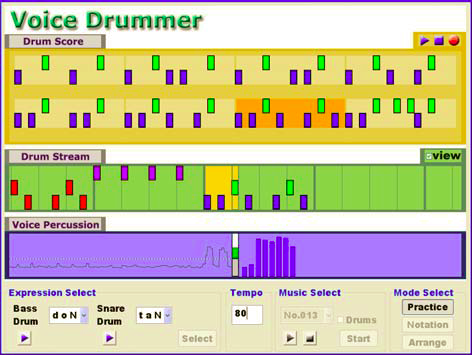
\includegraphics[height=5cm]{fig/VoiceDrummer.png}
		\caption{An example voice drummers practice adaption-mode}
		\label{VoiceDrummer}
	\end{center}
\end{figure}
\\
Onomatopoeic refers to words that phonetically imitates, or resembles the source of the described sound e.g. classifying 'Meow' as a sound a cat would make. Thus, making it easy for a layman to understand, and use Voice Drummer by uttering \textit{don-don} to generate a Bass Drum, and \textit{ta-ta} to generate a snare drum. These are transcribed into phonemic representations through a pronunciation dictionary which will recognize and
 output the correct corresponding output in real-time.

\subsection{ MATConcat }
In "MATConcat: An Application for Exploring Concatenative Sound Synthesis Using MATLAB"  By Bob L. Sturm, such an application has been made for Matlab. Here the method feature Concatenative sound synthesis is used, this methods will approximate a 'target' sound / input sound from a 'corpus' sound / database of sounds, the sound to use from the database is chosen from analysis of corpus sound and target to where they are matching most to some degree that can be set in the program (Sturm, 2004). The matching makes use of different parameters to make the choice of what is matching most. What degree of matching that the program will accept can be set in the interface and also what to do when the sound falls outside that degree (Sturm, 2004).

\subsection{ CataRT }
Another project called cataRT is using a similar method but in this project you can explore the analyzed data as they are shown in a space and as one navigates around in the space (cataRT, 2012). The space that one can navigate around in is comparable to what is described as the corpus or database in the MATConcat example, see figure0.1 for an better idea of how the interface looks like, this project is also implemented using a different platform that of maxMSP instead of MatLab.
\begin{figure}[h]
	\begin{center}
		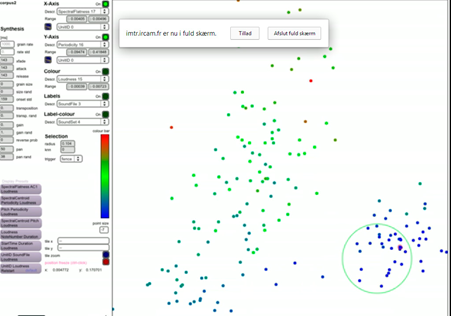
\includegraphics[height=5cm]{fig/cataRT.png}
		\caption{cataRT}
		\label{cataRT picture form video of cataRT showing the interface.}
	\end{center}
\end{figure} 
These methods could be using to make a voice imitate an instrument if a database was to be made with a given instrument, then by using this method it will be possible to analyze the input voice and find the closets sound from the database of the instrument sounds. Some analysis criteria would be needed to find the right database sound e.g. the pitch. 

\subsection{ Voice Band }
\begin{figure}[h]
	\begin{center}
		\includegraphics[height=5cm]{fig/voiceband.png}
		\caption{Voice Band}
		\label{VoiceBand}
	\end{center}
\end{figure}

Voice Band is an iPhone application by WaveMachine Labs which alters your voice into sampled instruments in real-time. It comes with a set of instruments to choose from including rhythm guitar, lead guitar, bass, sax, synthesizers, organ, drums and microphone, but there are other instruments and expansions available for purchase in the Voice Band store, e.g. other drum kits or strings. The target users are, according to WaveMachine Labs’ website and demo videos, songwriters who want an idea or arrangement down quickly; they call it a “portable musical scratch board”. However, it might also appeal and inspire anyone else interested in music, who wants to have fun. 

For every instrument, excluding the drums and cymbals, the system detects the pitch of the voice, and changes that into an instrumental output. To avoid distortion or unwanted noise, one will get the best results by using a pair of headphones, and staying in a quiet environment, because the system is very sensitive sound. It is also recommended to use solid, pure tones with no vibrato to reach a more accurate output, and to sing with hard consonants such as ba or da, because Voice Band recognizes the start of a sound, and it is therefore easier to detect.  

As for the drums, they are divided into kick/snare (two-in-one), hi-hat and crash. The kick and snare drums are together, where quiet will output kick, and loud notes will output snare. However there is the possibility to adjust the sensibility on a trigger in settings, such that only kick or only snare will be outputted, not depending on the loudness of the note. This way it is possible to record kick and snare separately as well. The hi-hat system works similarly in which soft notes produces a closed hi-hat and loud notes produces an open hi-hat. Crash is for itself. For all drums, and most of the other instruments, one can adjust reverberation and volume. 
All instruments and singing will have to be recorded separately, but on the same track. After having recorded an instrument, it will play back the previous recorded sounds while recording another one. It is possible to undo the last take without having to delete everything, but if you want to edit some of the first recordings this is not possible.  You cannot go back and change or edit the whole arrangement. It converts the samples into a MP3 file, which can be sent to an e-mail. 
